\section{Manual linguistic analysis}

This section describes manual marking of the use case steps parts on the \emph{City map} project. 
It explains assigning of the \emph{action type} of the step and binding of the \emph{text ranges} and \emph{action parts}.

\subsection{\emph{City map} project preparation}
We will reuse bundled project \emph{City map} and enhance contained use case \emph{Select city on map}. 

Import project \emph{cityMap} from \emph{exampleProjects} directory and open \emph{Select city on map} use case.

Select first use case step. In sentence analysis view set \emph{Action type} to \emph{To system}
becouse step sentence \emph{"The user opens the map web page"} describes communication of actor and system initiated by actor.

\begin{figure}[ht]
  \centering
  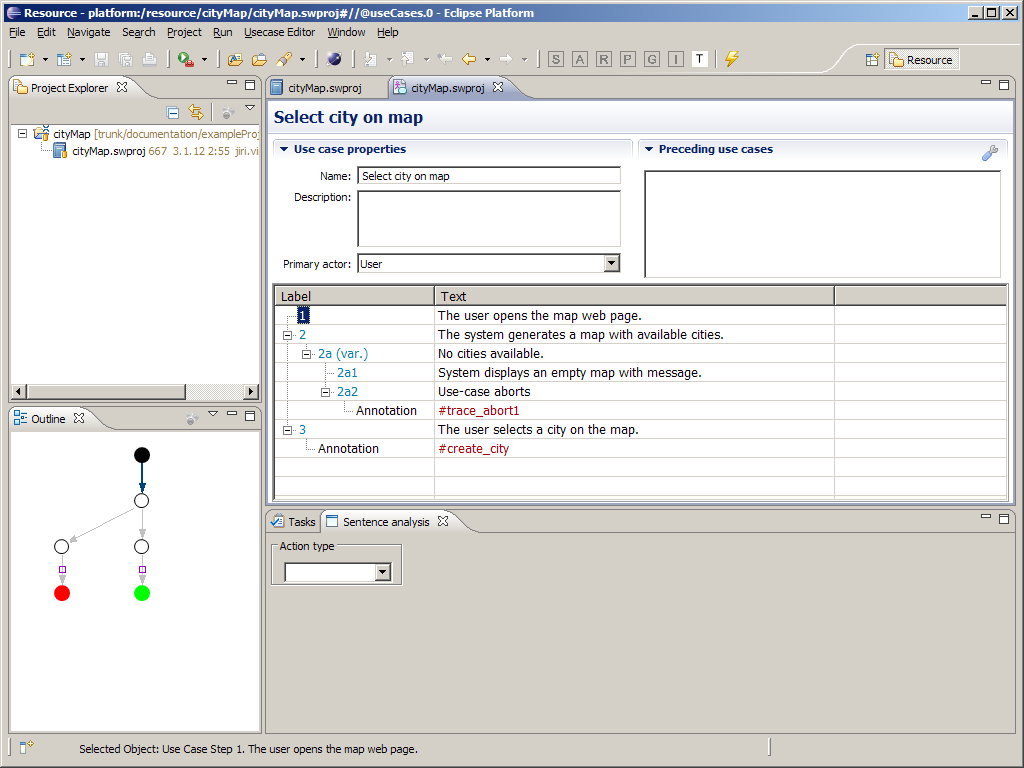
\includegraphics[height=280pt]{images/manual-analysis/step1-action-not-selected}
  \caption{Use case step before action specification}
  \label{fig:reprotoolUCEditor}
\end{figure}

Click on the first use case step and notice that boxes in \emph{Sentence analysis view} appeared and three icons in application toolbar got enabled.

\begin{figure}[ht]
  \centering
  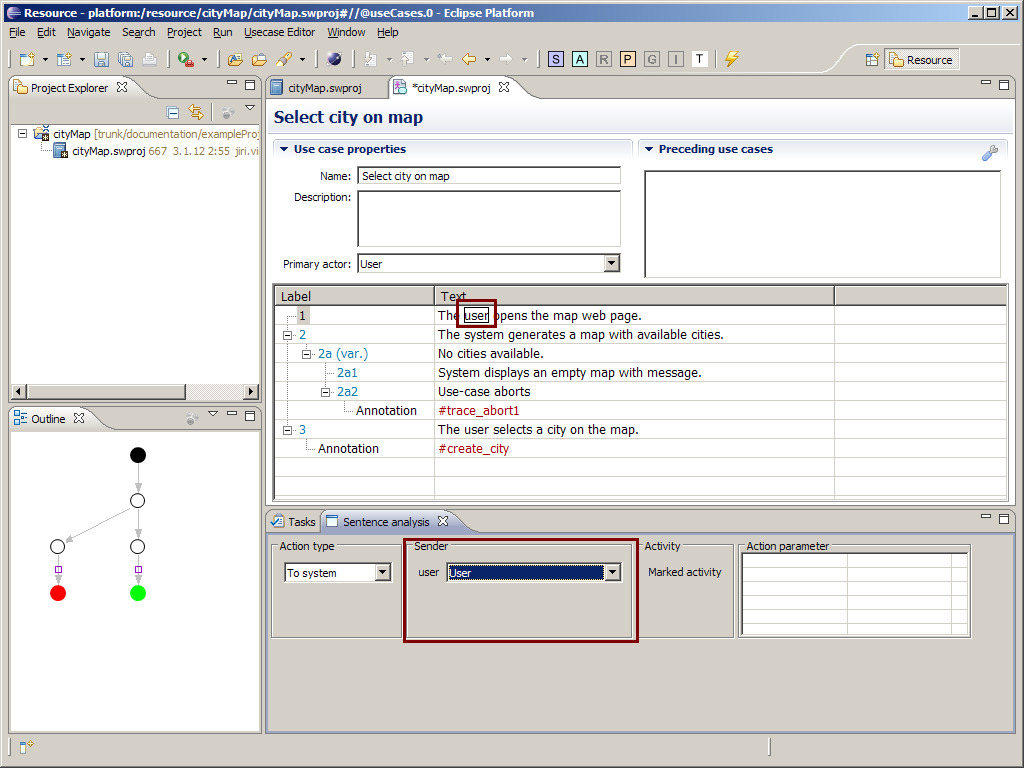
\includegraphics[height=280pt]{images/manual-analysis/step1-action-selected}
  \caption{\emph{To system} action specified}
  \label{fig:reprotoolUCEditor}
\end{figure}

Click into second column, select with mouse word "user" and click on "S" toolbar button. Border appears around the word and \emph{Sender} box in \emph{Sentence analysis view} now contains word "user". We call this \emph{textrange} selection. Now select in \emph{Sender} combobox item \emph{"User"}. This combobox is filled with actors contained in project.

\begin{figure}[ht]
  \centering
  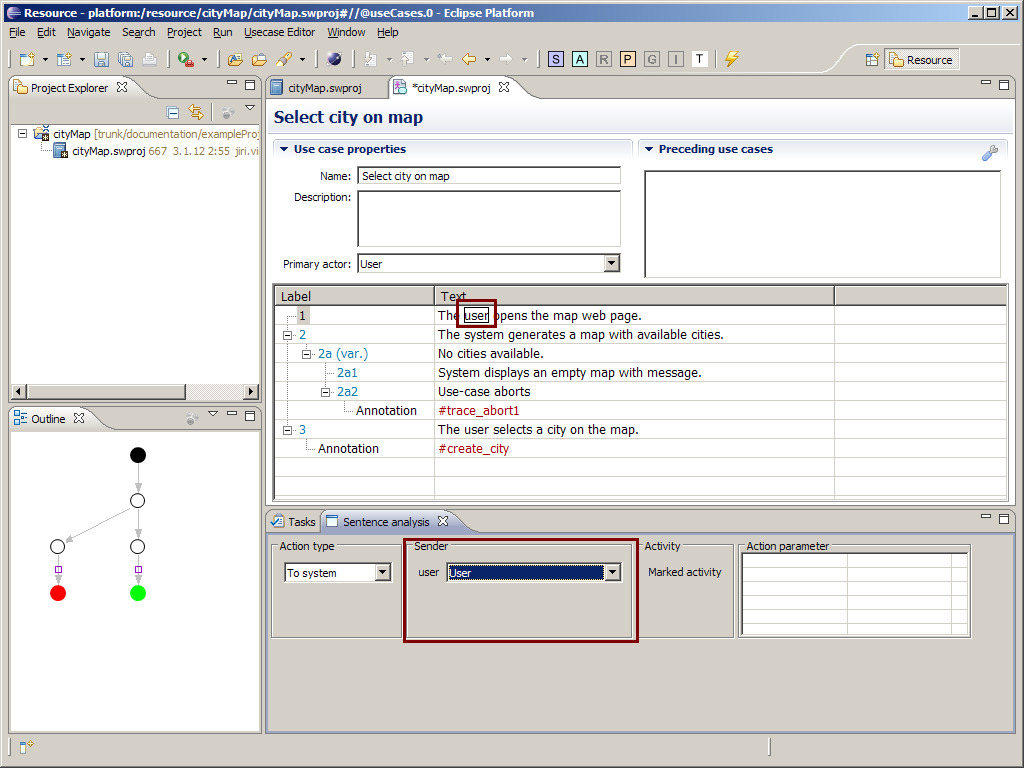
\includegraphics[height=280pt]{images/manual-analysis/step1-sender-selected}
  \caption{\emph{Sender} selected}
  \label{fig:reprotoolUCEditor}
\end{figure}

Similarly one can mark \emph{Activity} and \emph{Action parameters}. Box for the \emph{action parameters} allows to add more than one \emph{action parameter} becouse multiple parameters are
allowed in the step sentence. 

Analogous approach allows to mark \emph{Receiver} in the \emph{To system} action ("R" icon), \emph{Goto target} in the \emph{Goto} action ("G" icon) or \emph{Include target} in \emph{Include use case} action ("I" icon). "T" icon allows to "erase" already marked text.
